%% Created by Maple 2017.1, Windows 10
%% Source Worksheet: MechModel_GreenCrane_Matlab_REV0.mw
%% Generated: Mon Jan 15 09:08:44 CET 2018
\documentclass{article}
\usepackage{maplestd2e}
\def\emptyline{\vspace{12pt}}
\begin{document}
\pagestyle{empty}
\DefineParaStyle{Maple Bullet Item}
\DefineParaStyle{Maple Heading 1}
\DefineParaStyle{Maple Warning}
\DefineParaStyle{Maple Heading 4}
\DefineParaStyle{Maple Heading 2}
\DefineParaStyle{Maple Heading 3}
\DefineParaStyle{Maple Dash Item}
\DefineParaStyle{Maple Error}
\DefineParaStyle{Maple Title}
\DefineParaStyle{Maple Text Output}
\DefineParaStyle{Maple Normal}
\DefineCharStyle{Maple 2D Output}
\DefineCharStyle{Maple 2D Input}
\DefineCharStyle{Maple Maple Input}
\DefineCharStyle{Maple 2D Math}
\DefineCharStyle{Maple Hyperlink}
\begin{Maple Normal}{
\begin{Maple Normal}{
\mapleinline{inert}{2d}{}{\[\displaystyle \]}
}\end{Maple Normal}
}\end{Maple Normal}
\begin{maplegroup}
\begin{mapleinput}
\mapleinline{active}{2d}{}{$$}
\raisebox{9.375in}{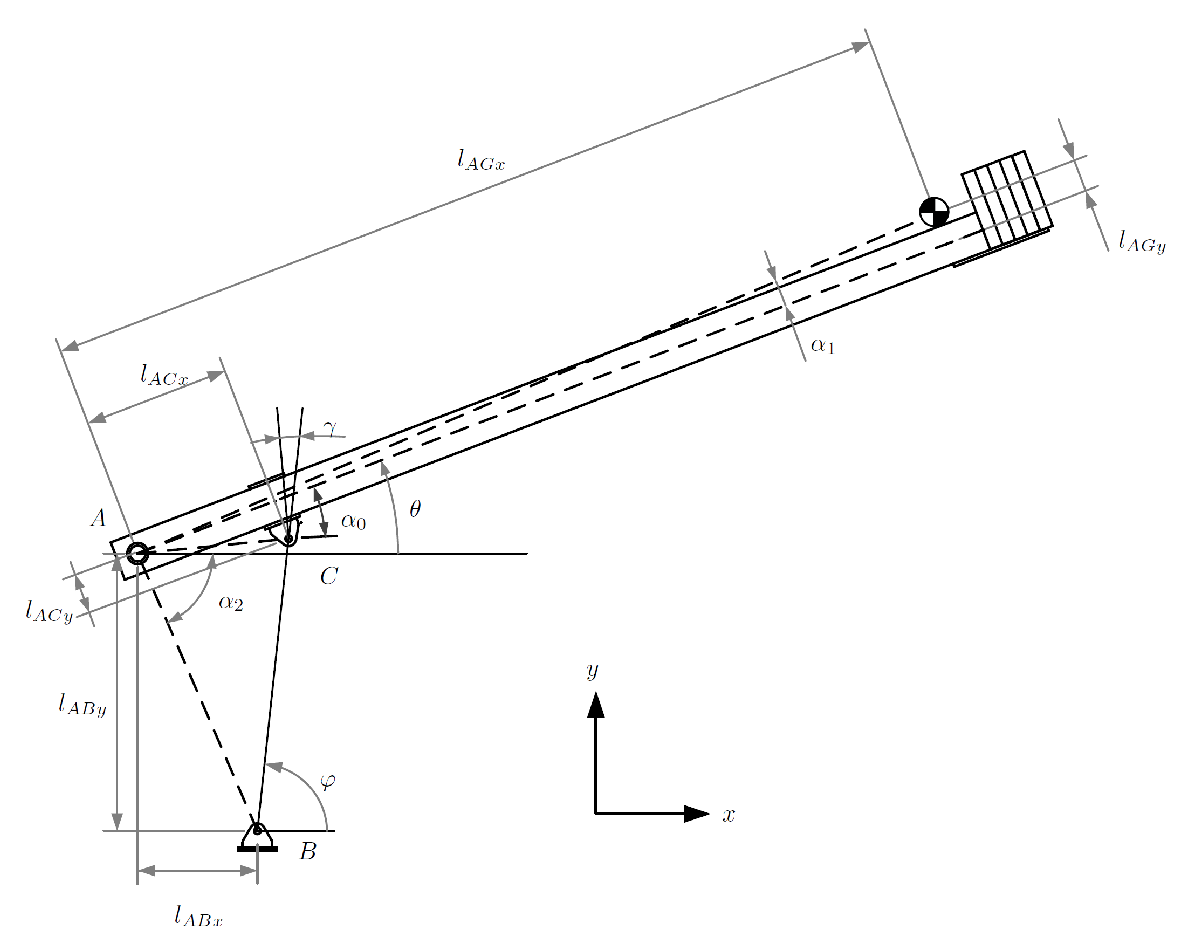
\includegraphics[keepaspectratio,totalheight=11.194444444444445in,angle=-90]{MechModel_GreenCrane_Matlab_REV0image0.eps}}\mapleinline{active}{1d}{}{}
\end{mapleinput}
\end{maplegroup}
\begin{maplegroup}
\begin{Maple Normal}{
\textbf{Mechanical Model og Green Crane @ UiA Laboratory}}\end{Maple Normal}

\end{maplegroup}
\begin{maplegroup}
\begin{mapleinput}
\mapleinline{active}{2d}{restart; 1}{\[\]}
\end{mapleinput}
\end{maplegroup}
\begin{maplegroup}
\begin{mapleinput}
\mapleinline{active}{2d}{with(LinearAlgebra); -1}{\[\]}
\end{mapleinput}
\end{maplegroup}
\begin{maplegroup}
\begin{mapleinput}
\mapleinline{active}{2d}{with(Physics); -1}{\[\]}
\end{mapleinput}
\end{maplegroup}
\begin{maplegroup}
\begin{Maple Normal}{
\textbf{Translational Position}}\end{Maple Normal}

\end{maplegroup}
\begin{maplegroup}
\begin{mapleinput}
\mapleinline{active}{2d}{R[p] := `<|>`(`<,>`(cos(theta[p](t)+alpha[1]), sin(theta[p](t)+alpha[1])), `<,>`(-sin(theta[p](t)+alpha[1]), cos(theta[p](t)+alpha[1]))); -1}{\[\]}
\end{mapleinput}
\end{maplegroup}
\begin{maplegroup}
\begin{mapleinput}
\mapleinline{active}{2d}{L[AG] := `<|>`(`<,>`(L[AGx], L[AGy])); -1}{\[\]}
\end{mapleinput}
\end{maplegroup}
\begin{maplegroup}
\begin{mapleinput}
\mapleinline{active}{2d}{x[cm] := Multiply(R[p], L[AG])[1, 1]; -1}{\[\]}
\end{mapleinput}
\end{maplegroup}
\begin{maplegroup}
\begin{mapleinput}
\mapleinline{active}{2d}{y[cm] := Multiply(R[p], L[AG])[2, 1]; -1}{\[\]}
\end{mapleinput}
\end{maplegroup}
\begin{maplegroup}
\begin{Maple Normal}{
\textbf{Translational Velocity}}\end{Maple Normal}

\end{maplegroup}
\begin{maplegroup}
\begin{mapleinput}
\mapleinline{active}{2d}{x[cmd] := diff(x[cm], t); -1}{\[\]}
\end{mapleinput}
\end{maplegroup}
\begin{maplegroup}
\begin{mapleinput}
\mapleinline{active}{2d}{y[cmd] := diff(y[cm], t); -1}{\[\]}
\end{mapleinput}
\end{maplegroup}
\begin{maplegroup}
\begin{mapleinput}
\mapleinline{active}{2d}{v[cm] := `<|>`(`<,>`(x[cmd], y[cmd])); -1}{\[\]}
\end{mapleinput}
\end{maplegroup}
\begin{maplegroup}
\begin{Maple Normal}{
\textbf{Angular Velocity}}\end{Maple Normal}

\end{maplegroup}
\begin{maplegroup}
\begin{mapleinput}
\mapleinline{active}{2d}{omega[p] := diff(theta[p](t), t); -1}{\[\]}
\end{mapleinput}
\end{maplegroup}
\begin{maplegroup}
\begin{Maple Normal}{
\textbf{Kinetic Energy}}\end{Maple Normal}

\end{maplegroup}
\begin{maplegroup}
\begin{mapleinput}
\mapleinline{active}{2d}{K[l] := (1/2)*m[cm]*Multiply(Transpose(v[cm]), v[cm])[1, 1]+(1/2)*j[cm]*omega[p]^2; -1}{\[\]}
\end{mapleinput}
\end{maplegroup}
\begin{maplegroup}
\begin{Maple Normal}{
\textbf{Potential Energy}}\end{Maple Normal}

\end{maplegroup}
\begin{maplegroup}
\begin{mapleinput}
\mapleinline{active}{2d}{P[l] := m[cm]*g*y[cm]; -1}{\[\]}
\end{mapleinput}
\end{maplegroup}
\begin{maplegroup}
\begin{Maple Normal}{
\textbf{Lagrangian}}\end{Maple Normal}

\end{maplegroup}
\begin{maplegroup}
\begin{mapleinput}
\mapleinline{active}{2d}{L[l] := K[l]-P[l]; -1}{\[\]}
\end{mapleinput}
\end{maplegroup}
\begin{maplegroup}
\begin{mapleinput}
\mapleinline{active}{2d}{tau[A1] := simplify(diff(diff(L[l], diff(theta[p](t), t)), t)-(diff(L[l], theta[p](t))), 'trig'); -1}{\[\]}
\end{mapleinput}
\end{maplegroup}
\begin{maplegroup}
\begin{Maple Normal}{
\textbf{Joint A Torque}}\end{Maple Normal}

\end{maplegroup}
\begin{maplegroup}
\begin{mapleinput}
\mapleinline{active}{2d}{tau[A] := collect(collect(collect(tau[A1], diff(theta[p](t), t, t)), diff(theta[p](t), t)), g); -1}{\[\]}
\end{mapleinput}
\end{maplegroup}
\begin{maplegroup}
\begin{Maple Normal}{
\textbf{Joint-to-Actuator Kinematics}}\end{Maple Normal}

\end{maplegroup}
\begin{maplegroup}
\begin{mapleinput}
\mapleinline{active}{2d}{restart; 1}{\[\]}
\end{mapleinput}
\end{maplegroup}
\begin{maplegroup}
\begin{mapleinput}
\mapleinline{active}{2d}{L[cyl] := x[p](t)+L[min]; -1}{\[\]}
\end{mapleinput}
\end{maplegroup}
\begin{maplegroup}
\begin{mapleinput}
\mapleinline{active}{2d}{alpha[4] := arccos((L[AB]^2+L[AC]^2-L[cyl]^2)/(2*L[AC]*L[AB]))-alpha[2]; -1}{\[\]}
\end{mapleinput}
\end{maplegroup}
\begin{maplegroup}
\begin{mapleinput}
\mapleinline{active}{2d}{theta[p] := alpha[4]+alpha[0]; -1}{\[\]}
\end{mapleinput}
\end{maplegroup}
\begin{maplegroup}
\begin{mapleinput}
\mapleinline{active}{2d}{diff(theta[p], t); -1}{\[\]}
\end{mapleinput}
\end{maplegroup}
\begin{maplegroup}
\begin{mapleinput}
\mapleinline{active}{2d}{diff(diff(theta[p], t), t); -1}{\[\]}
\end{mapleinput}
\end{maplegroup}
\begin{maplegroup}
\begin{Maple Normal}{
\textbf{Simplified Expressions}}\end{Maple Normal}

\end{maplegroup}
\begin{maplegroup}
\begin{mapleinput}
\mapleinline{active}{2d}{theta[d] := 2*L[cyl]*x[d]/(L[AC]*L[AB]*sqrt(4-(L[AB]^2+L[AC]^2-L[cyl]^2)^2/(L[AC]^2*L[AB]^2))); -1}{\[\]}
\end{mapleinput}
\end{maplegroup}
\begin{maplegroup}
\begin{mapleinput}
\mapleinline{active}{2d}{theta[dd] := 2*x[d]^2/(L[AC]*L[AB]*sqrt(4-(L[AB]^2+L[AC]^2-L[cyl]^2)^2/(L[AC]^2*L[AB]^2)))+2*L[cyl]*x[dd]/(L[AC]*L[AB]*sqrt(4-(L[AB]^2+L[AC]^2-L[cyl]^2)^2/(L[AC]^2*L[AB]^2)))-4*L[cyl]^2*x[d]^2*(L[AB]^2+L[AC]^2-L[cyl]^2)/(L[AC]^3*L[AB]^3*(4-(L[AB]^2+L[AC]^2-L[cyl]^2)^2/(L[AC]^2*L[AB]^2))^(3/2)); -1}{\[\]}
\end{mapleinput}
\end{maplegroup}
\begin{maplegroup}
\begin{mapleinput}
\mapleinline{active}{2d}{restart; 1}{\[\]}
\end{mapleinput}
\end{maplegroup}
\begin{maplegroup}
\begin{mapleinput}
\mapleinline{active}{2d}{tau[A] := (cos(theta[p]+alpha[1])*L[AGx]*m[cm]-sin(theta[p]+alpha[1])*L[AGy]*m[cm])*g+(L[AGx]^2*m[cm]+L[AGy]^2*m[cm]+j[cm])*theta[dd]; -1}{\[\]}
\end{mapleinput}
\end{maplegroup}
\begin{maplegroup}
\begin{Maple Normal}{
\textbf{Torque Arm}}\end{Maple Normal}

\end{maplegroup}
\begin{maplegroup}
\begin{mapleinput}
\mapleinline{active}{2d}{L[cyl] := x[p]+L[min]; -1}{\[\]}
\end{mapleinput}
\end{maplegroup}
\begin{maplegroup}
\begin{Maple Normal}{
\textbf{Relevant Angles}}\end{Maple Normal}

\end{maplegroup}
\begin{maplegroup}
\begin{mapleinput}
\mapleinline{active}{2d}{alpha[0] := arctan(L[ACy]/L[ACx]); -1}{\[\]}
\end{mapleinput}
\end{maplegroup}
\begin{maplegroup}
\begin{mapleinput}
\mapleinline{active}{2d}{alpha[1] := arctan(L[AGy]/L[AGx]); -1}{\[\]}
\end{mapleinput}
\end{maplegroup}
\begin{maplegroup}
\begin{mapleinput}
\mapleinline{active}{2d}{alpha[2] := arctan(L[ABy]/L[ABx]); -1}{\[\]}
\end{mapleinput}
\end{maplegroup}
\begin{maplegroup}
\begin{mapleinput}
\mapleinline{active}{2d}{alpha[3] := arccos((L[AB]^2-L[AC]^2+L[cyl]^2)/(2*L[cyl]*L[AB])); -1}{\[\]}
\end{mapleinput}
\end{maplegroup}
\begin{maplegroup}
\begin{mapleinput}
\mapleinline{active}{2d}{alpha[4] := arccos((L[AB]^2+L[AC]^2-L[cyl]^2)/(2*L[AC]*L[AB]))-alpha[2]; -1}{\[\]}
\end{mapleinput}
\end{maplegroup}
\begin{maplegroup}
\begin{mapleinput}
\mapleinline{active}{2d}{theta[p] := alpha[4]+alpha[0]; -1}{\[\]}
\end{mapleinput}
\end{maplegroup}
\begin{maplegroup}
\begin{mapleinput}
\mapleinline{active}{2d}{theta[d] := 2*L[cyl]*x[d]/(L[AC]*L[AB]*sqrt(4-(L[AB]^2+L[AC]^2-L[cyl]^2)^2/(L[AC]^2*L[AB]^2))); -1}{\[\]}
\end{mapleinput}
\end{maplegroup}
\begin{maplegroup}
\begin{mapleinput}
\mapleinline{active}{2d}{theta[dd] := 2*x[d]^2/(L[AC]*L[AB]*sqrt(4-(L[AB]^2+L[AC]^2-L[cyl]^2)^2/(L[AC]^2*L[AB]^2)))+2*L[cyl]*x[dd]/(L[AC]*L[AB]*sqrt(4-(L[AB]^2+L[AC]^2-L[cyl]^2)^2/(L[AC]^2*L[AB]^2)))-4*L[cyl]^2*x[d]^2*(L[AB]^2+L[AC]^2-L[cyl]^2)/(L[AC]^3*L[AB]^3*(4-(L[AB]^2+L[AC]^2-L[cyl]^2)^2/(L[AC]^2*L[AB]^2))^(3/2)); -1}{\[\]}
\end{mapleinput}
\end{maplegroup}
\begin{maplegroup}
\begin{mapleinput}
\mapleinline{active}{2d}{L[arm] := L[AB]*sin(alpha[3]); -1}{$$}
\mapleinline{active}{2d}{}{$$}
\end{mapleinput}
\end{maplegroup}
\begin{maplegroup}
\begin{Maple Normal}{
\textbf{Cylinder Output Force}}\end{Maple Normal}

\end{maplegroup}
\begin{maplegroup}
\begin{mapleinput}
\mapleinline{active}{2d}{F[cyl1] := simplify(solve(tau[A] = L[arm]*F[cyl], F[cyl]), 'symbolic'); -1}{\[\]}
\end{mapleinput}
\end{maplegroup}
\begin{maplegroup}
\begin{Maple Normal}{
\textbf{Generalized Force Balance Formulation}}\end{Maple Normal}

\end{maplegroup}
\begin{maplegroup}
\begin{mapleinput}
\mapleinline{active}{2d}{M[eq] := -(4*(L[AGx]^2*L[cyl]*m[cm]+L[AGy]^2*L[cyl]*m[cm]+L[cyl]*j[cm]))*L[cyl]/((L[AB]-L[cyl]-L[AC])*(L[AB]-L[cyl]+L[AC])*(L[cyl]+L[AB]+L[AC])*(L[cyl]+L[AB]-L[AC])); -1}{\[\]}
\end{mapleinput}
\end{maplegroup}
\begin{maplegroup}
\begin{mapleinput}
\mapleinline{active}{2d}{C[eq] := (4*((L[AGx]^2+L[AGy]^2)*m[cm]+j[cm]))*L[cyl]*(-L[AB]^2+L[AC]^2+L[cyl]^2)*(L[AB]^2-L[AC]^2+L[cyl]^2)/((L[cyl]-L[AC]-L[AB])^2*(L[cyl]+L[AC]-L[AB])^2*(L[cyl]+L[AB]+L[AC])^2*(L[cyl]+L[AB]-L[AC])^2); -1}{\[\]}
\end{mapleinput}
\end{maplegroup}
\begin{maplegroup}
\begin{mapleinput}
\mapleinline{active}{2d}{G[eq] := -2*sqrt(-(L[cyl]+L[AC]-L[AB])*(L[cyl]-L[AC]-L[AB])*(L[cyl]+L[AB]-L[AC])*(L[cyl]+L[AB]+L[AC]))*g*m[cm]*(cos(arccos((1/2)*(L[AB]^2+L[AC]^2-L[cyl]^2)/(L[AC]*L[AB]))-alpha[2]+alpha[0]+alpha[1])*L[AGx]-sin(arccos((1/2)*(L[AB]^2+L[AC]^2-L[cyl]^2)/(L[AC]*L[AB]))-alpha[2]+alpha[0]+alpha[1])*L[AGy])*L[cyl]/((L[cyl]+L[AC]-L[AB])*(L[cyl]-L[AC]-L[AB])*(L[cyl]+L[AB]-L[AC])*(L[cyl]+L[AB]+L[AC])); -1}{\[\]}
\end{mapleinput}
\end{maplegroup}
\begin{maplegroup}
\begin{mapleinput}
\mapleinline{active}{2d}{F[cyl] := C[eq]*x[d]^2+M[eq]*x[dd]+G[eq]; -1}{$$}
\mapleinline{active}{2d}{}{$$}
\end{mapleinput}
\end{maplegroup}
\begin{maplegroup}
\begin{Maple Normal}{
\textbf{Verification of Generalized Force Balance Formulation}}\end{Maple Normal}

\end{maplegroup}
\begin{maplegroup}
\begin{mapleinput}
\mapleinline{active}{2d}{factor(F[cyl1]-F[cyl])}{\[{\it factor} \left( F_{{{\it cyl1}}}-F_{{{\it cyl}}} \right) \]}
\end{mapleinput}
\mapleresult
\begin{maplelatex}
\mapleinline{inert}{2d}{0}{\[\displaystyle 0\]}
\end{maplelatex}
\end{maplegroup}
\begin{maplegroup}
\begin{Maple Normal}{
\textbf{Lengths \& Mass Properties}}\end{Maple Normal}

\end{maplegroup}
\begin{maplegroup}
\begin{mapleinput}
\mapleinline{active}{2d}{L[AGx] := L_AGx; -1}{\[\]}
\end{mapleinput}
\end{maplegroup}
\begin{maplegroup}
\begin{mapleinput}
\mapleinline{active}{2d}{L[AGy] := L_AGy; -1}{\[\]}
\end{mapleinput}
\end{maplegroup}
\begin{maplegroup}
\begin{mapleinput}
\mapleinline{active}{2d}{L[ACx] := L_ACx; -1}{\[\]}
\end{mapleinput}
\end{maplegroup}
\begin{maplegroup}
\begin{mapleinput}
\mapleinline{active}{2d}{L[ACy] := L_ACy; -1}{\[\]}
\end{mapleinput}
\end{maplegroup}
\begin{maplegroup}
\begin{mapleinput}
\mapleinline{active}{2d}{L[ABx] := L_ABx; -1}{\[\]}
\end{mapleinput}
\end{maplegroup}
\begin{maplegroup}
\begin{mapleinput}
\mapleinline{active}{2d}{L[ABy] := L_ABy; -1}{\[\]}
\end{mapleinput}
\end{maplegroup}
\begin{maplegroup}
\begin{mapleinput}
\mapleinline{active}{2d}{L[AB] := L_AB; -1}{\[\]}
\end{mapleinput}
\end{maplegroup}
\begin{maplegroup}
\begin{mapleinput}
\mapleinline{active}{2d}{L[AC] := L_AC; -1}{\[\]}
\end{mapleinput}
\end{maplegroup}
\begin{maplegroup}
\begin{mapleinput}
\mapleinline{active}{2d}{L[AG] := L_AG; -1}{\[\]}
\end{mapleinput}
\end{maplegroup}
\begin{maplegroup}
\begin{mapleinput}
\mapleinline{active}{2d}{m[cm] := m_cm; -1}{\[\]}
\end{mapleinput}
\end{maplegroup}
\begin{maplegroup}
\begin{mapleinput}
\mapleinline{active}{2d}{x[p] := x; -1}{\[\]}
\end{mapleinput}
\end{maplegroup}
\begin{maplegroup}
\begin{mapleinput}
\mapleinline{active}{2d}{j[cm] := J_cm; -1}{\[\]}
\end{mapleinput}
\end{maplegroup}
\begin{maplegroup}
\begin{mapleinput}
\mapleinline{active}{2d}{L[min] := L_min; -1}{\[\]}
\end{mapleinput}
\end{maplegroup}
\begin{maplegroup}
\begin{Maple Normal}{
\textbf{Conversion to Matlab Code}}\end{Maple Normal}

\end{maplegroup}
\begin{maplegroup}
\begin{mapleinput}
\mapleinline{active}{2d}{CodeGeneration['Matlab'](G[eq])}{\[{\it CodeGeneration}_{{'Matlab'}} \left( G_{{{\it eq}}} \right) \]}
\end{mapleinput}
\mapleresult
cg = -0.2e1 * sqrt(-(x - L\_AB + L\_min + L\_AC) * (x + L\_min - L\_AC - L\_AB) * (x + L\_AB + L\_min - L\_AC) * (x + L\_AB + L\_min + L\_AC)) * g * m\_cm * (cos(acos((L\_AB \symbol{94} 2 + L\_AC \symbol{94} 2 - (x + L\_min) \symbol{94} 2) / L\_AC / L\_AB / 0.2e1) - atan(L\_ABy / L\_ABx) + atan(L\_ACy / L\_ACx) + atan(L\_AGy / L\_AGx)) * L\_AGx - sin(acos((L\_AB \symbol{94} 2 + L\_AC \symbol{94} 2 - (x + L\_min) \symbol{94} 2) / L\_AC / L\_AB / 0.2e1) - atan(L\_ABy / L\_ABx) + atan(L\_ACy / L\_ACx) + atan(L\_AGy / L\_AGx)) * L\_AGy) * (x + L\_min) / (x - L\_AB + L\_min + L\_AC) / (x + L\_min - L\_AC - L\_AB) / (x + L\_AB + L\_min - L\_AC) / (x + L\_AB + L\_min + L\_AC);
\end{maplegroup}
\begin{maplegroup}
\begin{mapleinput}
\mapleinline{active}{2d}{CodeGeneration['Matlab'](M[eq])}{\[{\it CodeGeneration}_{{'Matlab'}} \left( M_{{{\it eq}}} \right) \]}
\end{mapleinput}
\mapleresult
cg0 = -4 * (L\_AGx \symbol{94} 2 * (x + L\_min) * m\_cm + L\_AGy \symbol{94} 2 * (x + L\_min) * m\_cm + (x + L\_min) * J\_cm) * (x + L\_min) / (-x + L\_AB - L\_min - L\_AC) / (-x + L\_AB - L\_min + L\_AC) / (x + L\_AB + L\_min + L\_AC) / (x + L\_AB + L\_min - L\_AC);
\end{maplegroup}
\begin{maplegroup}
\begin{mapleinput}
\mapleinline{active}{2d}{CodeGeneration['Matlab'](C[eq])}{\[{\it CodeGeneration}_{{'Matlab'}} \left( C_{{{\it eq}}} \right) \]}
\end{mapleinput}
\mapleresult
cg1 = 4 * ((L\_AGx \symbol{94} 2 + L\_AGy \symbol{94} 2) * m\_cm + J\_cm) * (x + L\_min) * (-L\_AB \symbol{94} 2 + L\_AC \symbol{94} 2 + (x + L\_min) \symbol{94} 2) * (L\_AB \symbol{94} 2 - L\_AC \symbol{94} 2 + (x + L\_min) \symbol{94} 2) / (x + L\_min - L\_AC - L\_AB) \symbol{94} 2 / (x - L\_AB + L\_min + L\_AC) \symbol{94} 2 / (x + L\_AB + L\_min + L\_AC) \symbol{94} 2 / (x + L\_AB + L\_min - L\_AC) \symbol{94} 2;
\end{maplegroup}
\begin{maplegroup}
\begin{mapleinput}
\mapleinline{active}{2d}{}{\[\]}
\end{mapleinput}
\end{maplegroup}
\begin{Maple Normal}{
\begin{Maple Normal}{
\mapleinline{inert}{2d}{}{\[\displaystyle \]}
}\end{Maple Normal}
}\end{Maple Normal}
\end{document}
